\section{Experiment Environments}
\label{sec:experiments}

In this section, we introduce the experiment environments to evaluate our approaches in this thesis. We first introduce FutureGrid, a distributed cloud platform and then WorkflowSim, a traced based simulator developed by us. 

\subsection{FutureGrid}
FutureGrid \cite{Fox2013FutureGrid} is a distributed, high-performance testbed that provides scientists with a set of computing resources to develop parallel, grid, and cloud applications. We used FutureGrid to evaluate our workflow partitioning algorithms in Chapter~\ref{chap:partitioning} and we also collected the traces of workflows that were run on FutureGrid to feed WorkflowSim such that it can simulate workflows with better accuracy. 

FutureGrid is built out of a number of clusters of different types and sizes that are interconnected with up to a 10GB Ethernet between its sites. In our experiments of workflow partitioning, we have used five execution sites including Indiana University (IU), University of Chicago (UC), San Diego Supercomputing Center (SDSC), Texas Advanced Computing Center (TACC), and University of Florida (UF). The FutureGrid policy allows us to launch 20 virtual machines in each site. Table~\ref{tab:model_clusters} shows the overview of these clusters. 

\begin{table}[h!]
\caption{Overview of the Clusters}
\label{tab:model_clusters}
\centering
\begin{tabular}{lrrrrrrr}
\hline
Site &  Name &  Nodes & CPUs & Cores &  RAM(GB) & Storage (TB)     \\\hline
IU & india & 128 & 256 & 1024 & 3072 & 335 \\
UC & hotel & 84 & 168 & 672 & 2016 & 120 \\
SDSC & sierra & 84 & 168 & 672 & 2688 & 96 \\
UF & foxtrot & 32 & 64 & 256 & 768 & 0 \\
TACC & alamo & 96 & 192 & 768 & 1152 & 30 \\\hline
\end{tabular}
\end{table} 



\subsection{WorkflowSim}

We have developed WorkflowSim as an open source workflow simulator that extends CloudSim \cite{Calheiros2011} by providing a workflow level support of simulation. It models workflows with an o-DAG model with support of an elaborate model of node failures, a model of delays occurring in the various levels of the WMS stack \cite{Chen2011}, the implementations of several most popular dynamic and static workflow schedulers (e.g., HEFT\cite{Topcuoglu2002} and MinMin\cite{Blythe2005}) and task clustering algorithms (e.g., runtime-based algorithms \cite{Chen2013b}, data-oriented algorithms \cite{Chen2013b} and fault tolerant clustering algorithms \cite{Chen2012}). Parameters are imported from traces of workflow executions that were run on FutureGrid~\cite{Fox2013FutureGrid}. 

%However, an accurate simulation framework for scientific workflows is required to generate reasonable results, particularly considering that the overall system overhead \cite{Chen2011} plays a significant role in the workflow’s runtime. 
In distributed systems, workflows may experience different types of overheads.  Since the causes of overheads differ, the overheads have diverse distributions and behaviors. For example, the time to run a post-script that checks the return status of a computation is usually a constant. However, queue delays incurred while tasks are waiting in a batch scheduling systems can vary widely. 
By classifying these workflow overheads in different layers and system components, our simulator can offer a more accurate result than simulators that do not include overheads in their system models.

What’s more, many researchers \cite{Zhang2004, Tang1990, Schroeder2006, Sahoo2004, Oppenheimer2002, McConnel1979} have emphasized the importance of fault tolerant design and concluded that the failure rates in modern distributed systems should not be ignored. A simulation with support of random failures with different distributions is implemented in WorkflowSim to promote such studies. 

Finally, progress in workflow research also requires a general-purpose framework that can support widely accepted features of workflows and optimization techniques. Existing simulators such as CloudSim/GridSim \cite{Calheiros2011} fail to provide fine granularity simulations of workflows. For example, they lack the support of task clustering. The simulation of task clustering requires two layers of execution model, on both task and job levels. It also requires a workflow-clustering engine that launches algorithms and heuristics to cluster tasks. Other techniques such as workflow partitioning and task retry are also ignored in these simulators. These features have been implemented in WorkflowSim. 

To the best of our knowledge, none of the current distributed system simulators support these rich-features and techniques. Below, we introduce our early work on simulating scientific workflows satisfying these requirements. We evaluate the performance of WorkflowSim with an example of task clustering. 

\subsubsection{Components and Functionalities}

\begin{figure}[!htb]
	\centering
	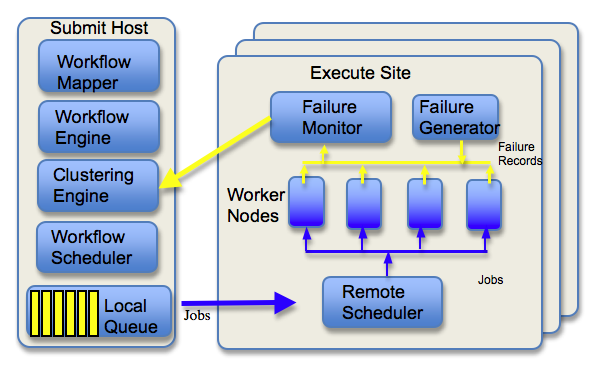
\includegraphics[width=0.6\linewidth]{figures/workflowsim/wfs_overview.png}
	\caption{Overview of WorkflowSim.}
	\label{fig:model_wfs}
\end{figure}

Deelman et. al. \cite{Deelman2009} have provided a survey of popular workflow systems for scientific applications and have classified their components into four categories: composition, mapping, execution, and provenance. Based on this survey, we identified the mandatory functionalities/components and designed the layers in our WorkflowSim. In our design as shown in Figure~\ref{fig:model_wfs}, we add multiple layers on top of the existing task scheduling layer of CloudSim, which include Workflow Mapper, Workflow Engine, Clustering Engine, Workflow Scheduler, Failure Generator and Failure Monitor etc. 

\begin{enumerate}

\item {Workflow Mapper} is used to import DAG files formatted in XML (called DAX in WorkflowSim) and other metadata information such as file size from Workflow Generator \cite{WorkflowGenerator}. Workflow Mapper creates a list of tasks and assigns these tasks to an execution site. A task is a program/activity that a user would like to execute. 

\item{Workflow Engine} manages tasks based on their dependencies between tasks to assure that a task may only be released when all of its parent tasks have completed successfully. Workflow Engine will only release free tasks to Clustering Engine. 

\item{Clustering Engine} merges tasks into jobs such that the scheduling overhead is reduced. A job is an atomic unit seen by the execution system, which contains multiple tasks to be executed in sequence or in parallel if applicable. Different to the clustering engine in Pegasus WMS, Clustering Engine in WorkflowSim also performs task reclustering in a faulty execution environment. The details will be introduced in Chapter \ref{chap:tolerance}. 

\item{Workflow Scheduler} is used to match jobs to a worker node based on the criteria selected by users. WorkflowSim relies on CloudSim to provide an accurate and reliable job-level execution model, such as time-shared model and space-shared model. However, WorkflowSim has introduced different layers of system overheads and failures, which improves the accuracy of simulation. 

\item{Failure Generator} is introduced to inject task/job failures at each execution site during the simulation. After the execution of each job, Failure Generator randomly generates task/job failures based on the distribution that a user has specified. 

\item{Failure Monitor} collects failure records (e.g., resource id, job id, task id) and returns these records to Clustering Engine to adjust the clustering strategies dynamically. 

\end{enumerate}




\subsubsection{Results and Validation}
We use task clustering as an example to illustrate the necessity of introducing system overheads into workflow simulation. The goal was to compare the simulated overall runtime of workflows in case the information of job runtime and system overheads are known and extracted from prior traces. 
In this example, we collected real traces generated by the Pegasus Workflow Management System while executing workflows on FutureGrid \cite{Fox2013FutureGrid}. We built an execution site with 20 worker nodes and we executed the Montage workflow five times in every single configuration of $clusters.num$, which is the maximum number of clustered jobs in a horizontal level. These five traces of workflow execution with the same $clusters.num$ is a training set or a validation set. 
%Partly illustrated by Figure 5, the results are stable enough to be used as a training set. 
We ran the Montage workflow with a size of 8-degree squares of sky. The workflow has 10,422 tasks and 57GB of overall data. We tried different $clusters.num$ from 20 to 100, leaving us 5 groups of data sets with each group having 5 workflow traces. 
First of all, we adopt a simple approach that selects a training set to train WorkflowSim and then use the same training set as validation set to compare the predicted overall runtime and the real overall runtime in the traces. We define accuracy in this section as the ratio between the predicted overall runtime and the real overall runtime:
\begin{equation} \label{eq:model_wfs_accuracy}
Accuracy=\frac{Predicted~Overall~Runtime}{Real~Overall~Runtime}
\end{equation}
 \begin{figure}[h!]
	\centering
    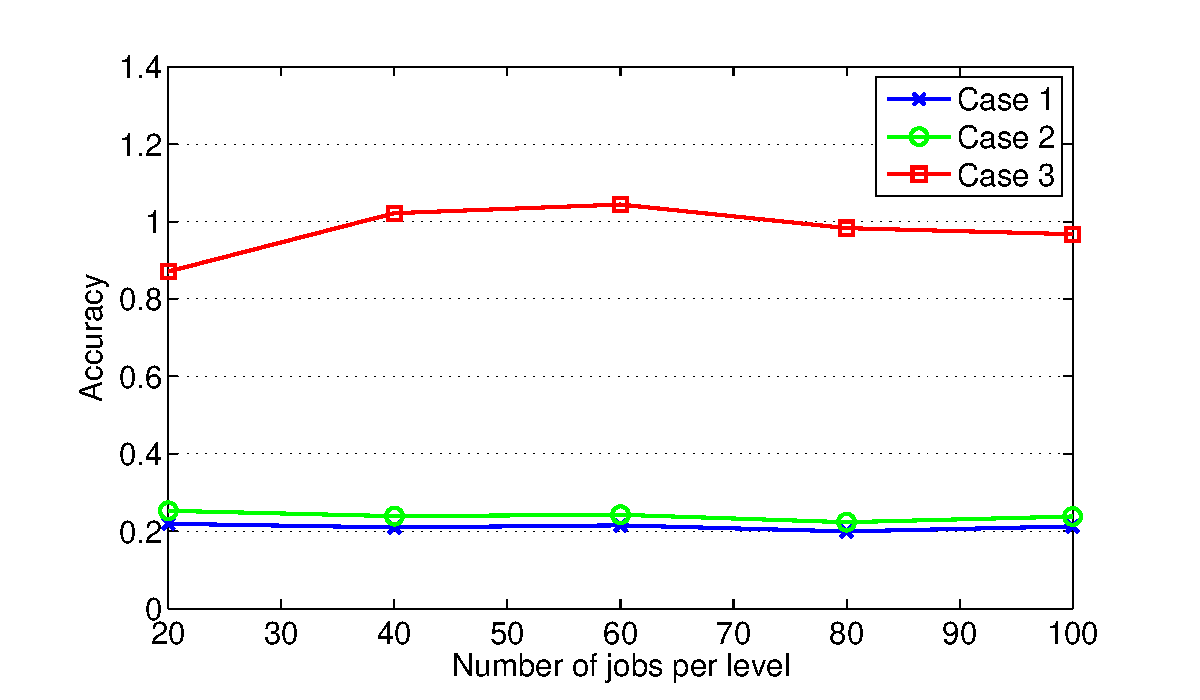
\includegraphics[width=0.7\textwidth]{figures/model/wfs_levels.eps}
    \caption{Performance of WorkflowSim with different support levels}
    \label{fig:model_wfs_levels}
\end{figure} 
 
%Performance of WorkflowSim with different support levels. 
To train WorkflowSim, from the traces of workflow execution (training sets), we extracted information about job runtime and overheads, such as average/distribution and, for example, whether it has a cyclic increase. We then added these parameters into the generation of system overheads and simulated them as close as possible to the real cases. 

To present an explicit comparison, we simulated the cases using WorkflowSim that has no consideration of workflow dependencies or overheads (Case 1), WorkflowSim with Workflow Engine that has considered the influence of dependencies but ignored system overheads (Case 2), and WorkflowSim, that has covered both aspects (Case 3). Intuitively, we expect that the order of the accuracy of them should be Case 3 $>$ Case 2 $>$ Case 1. 

Fig~\ref{fig:model_wfs_levels} shows that the performance of WorkflowSim with different support levels is consistent to our expectation. The accuracy of Case 3 is quite close to but not equal to 1.0 in most points. The reason is that to simulate workflows, WorkflowSim has to simplify models with a few parameters, such as the average value and the distribution type. It is not efficient to recur every overhead as is present in the real traces. It is also impossible to do so since the traces within the same training set may have much variance in each run. Fig~\ref{fig:model_wfs_levels} also shows that the accuracy of both Case 1 and Case 2 are much lower than that of Case 3. The reason is that it ignores both dependencies and multiple layers of overheads. By ignoring data dependencies, it releases tasks that are not supposed to run since their parents have not completed (a real workflow system should never do that) and thereby reducing the overall runtime. At the same time, it executes jobs/tasks irrespective of the actual overheads, which further reduces the simulated overall runtime. In Case 2, with the help of Workflow Engine, WorkflowSim is able to control the release of tasks and thereby the simulated overall runtime is closer to the real traces. However, since it has ignored most overheads, jobs are completed and returned earlier than that in real traces. The low accuracy of Case 1 and Case 2 confirms the necessity of introducing overhead design into our simulator. 


\section{Summary}

In this chapter, we have introduced the workflow and system models including an overhead-aware DAG model that we have proposed, the execution environments including a workflow simulator that we have developed, and the workflows used in this thesis. As indicated by Table~\ref{tab:model_clusters}, resources such the data storage are limited in a data center. In next chapter, we will introduce the first proposed approach called Workflow Partitioning to address the optimization of workflows with resource constraints.